	%====================================================================================================
	% ?????
	%====================================================================================================
	% TCC
	%----------------------------------------------------------------------------------------------------
	% Autor				: Jasane Schio
	% Orientador		: Gedson Faria
	% Co-Orientador		: Angelo Darcy
	% Instituição 		: UFMS - Universidade Federal do Mato Grosso do Sul
	% Departamento		: CPCX - Sistema de Informação
	%----------------------------------------------------------------------------------------------------
	% Data de criação	: 01 de Outubro de 2015
	%====================================================================================================
	
	\definecolor{dkgreen}{rgb}{0,0.6,0}
	\definecolor{gray}{rgb}{0.5,0.5,0.5}
	\definecolor{mauve}{rgb}{0.58,0,0.82}
	
	\lstset{frame=tb,
		language=C++,
		aboveskip=3mm,
		belowskip=3mm,
		showstringspaces=false,
		columns=flexible,
		basicstyle={\small\ttfamily},
		numbers=none,
		numberstyle=\tiny\color{gray},
		keywordstyle=\color{blue},
		commentstyle=\color{dkgreen},
		stringstyle=\color{mauve},
		breaklines=true,
		breakatwhitespace=true,
		tabsize=3
	}
	\chapter{Metodologia e Desenvolvimento} \label{Cap:Processamento}
	
			Para o desenvolvimento foi escolhida a biblioteca OpenCV por ser OpenSource, multiplataforma, uma grande quantidade de métodos e algoritmos já implementados	e pelo seu rápido desempenho de máquina.
			A linguagem escolhida para o desenvolvimento foi o C++ pois é uma linguagem de programação compilada, o que torna sua execução mais rápida que as linguagem interpretadas, tendo assim grande desempenho e por ser uma linguagem orientada objeto. 
			
			O sistema desenvolvido é separado em duas partes: Processamento e Interface Gráfica.
			A parte de Processamento é onde são feitas as partes de aquisição de imagem, processamento de imagem, conversão de imagem para modelo de cor HSV, seleção de pontos de cor e contagem de ocorrência de cor. Já a interface gráfica, é a onde ocorre a entrada do usuário para assim ser feita a calibração manual de mínimos e máximos de cada cor.
		
	
	Passos do projeto:
	\begin{description}
		\item[Aquisição de imagens em vídeo:] Nesse passo as imagem são adquiridas via câmera USB.
		
		\item[Identificação de Objetos:]
				 Durante o processo de aquisição de imagem são selecionados os objetos, quais serão usados como base para a detecção de máximos e mínimos de cores.
		\item [Cálculo de Mínimos e Máximos:]
		 Nessa etapa são levados em consideração os objetos teste. A imagem é "varrida"  por pixel na localidade dos objetos-teste e assim são salvos seus valores e feito a contagem de ocorrências de cada cor.		
	\end{description}


	\section{Projeto}
	\subsection{Organização do Projeto}
	 O projeto está sendo sendo desenvolvido na IDE QT Creator e está separada em três pastas. Na pasta Headers estão os arquivos de cabeçalho(.h) onde estão as declarações dos métodos e variáveis usados nas classes  executáveis. Já na pasta Sources estão os arquivos fonte(.cpp), são nesses arquivos que os métodos declarados nos arquivos da pasta Header são implementados. Na pasta Forms está o arquivo de interface gráfica(.ui) usada no projeto.
	 
	\begin{figure}[!h]
		\centering
		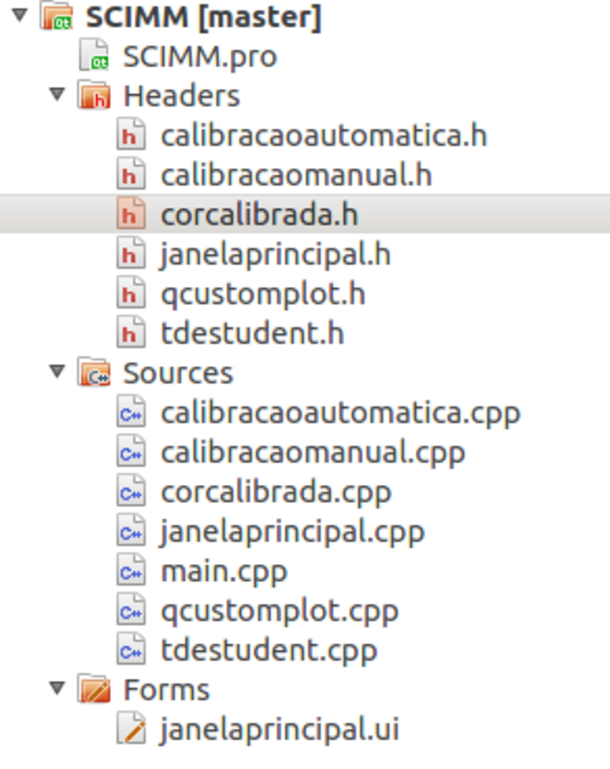
\includegraphics[width=0.15\textwidth]{organizacaoProjeto.pdf}
		\caption{Organização das pastas do projeto}
		\label{Organizacao do Projeto}
	\end{figure}
	 A seguir mostrarei o Diagrama de Classes e explicarei os métodos que fazem parte das classes.
	 \begin{figure}[!h]
	 	\centering
	 	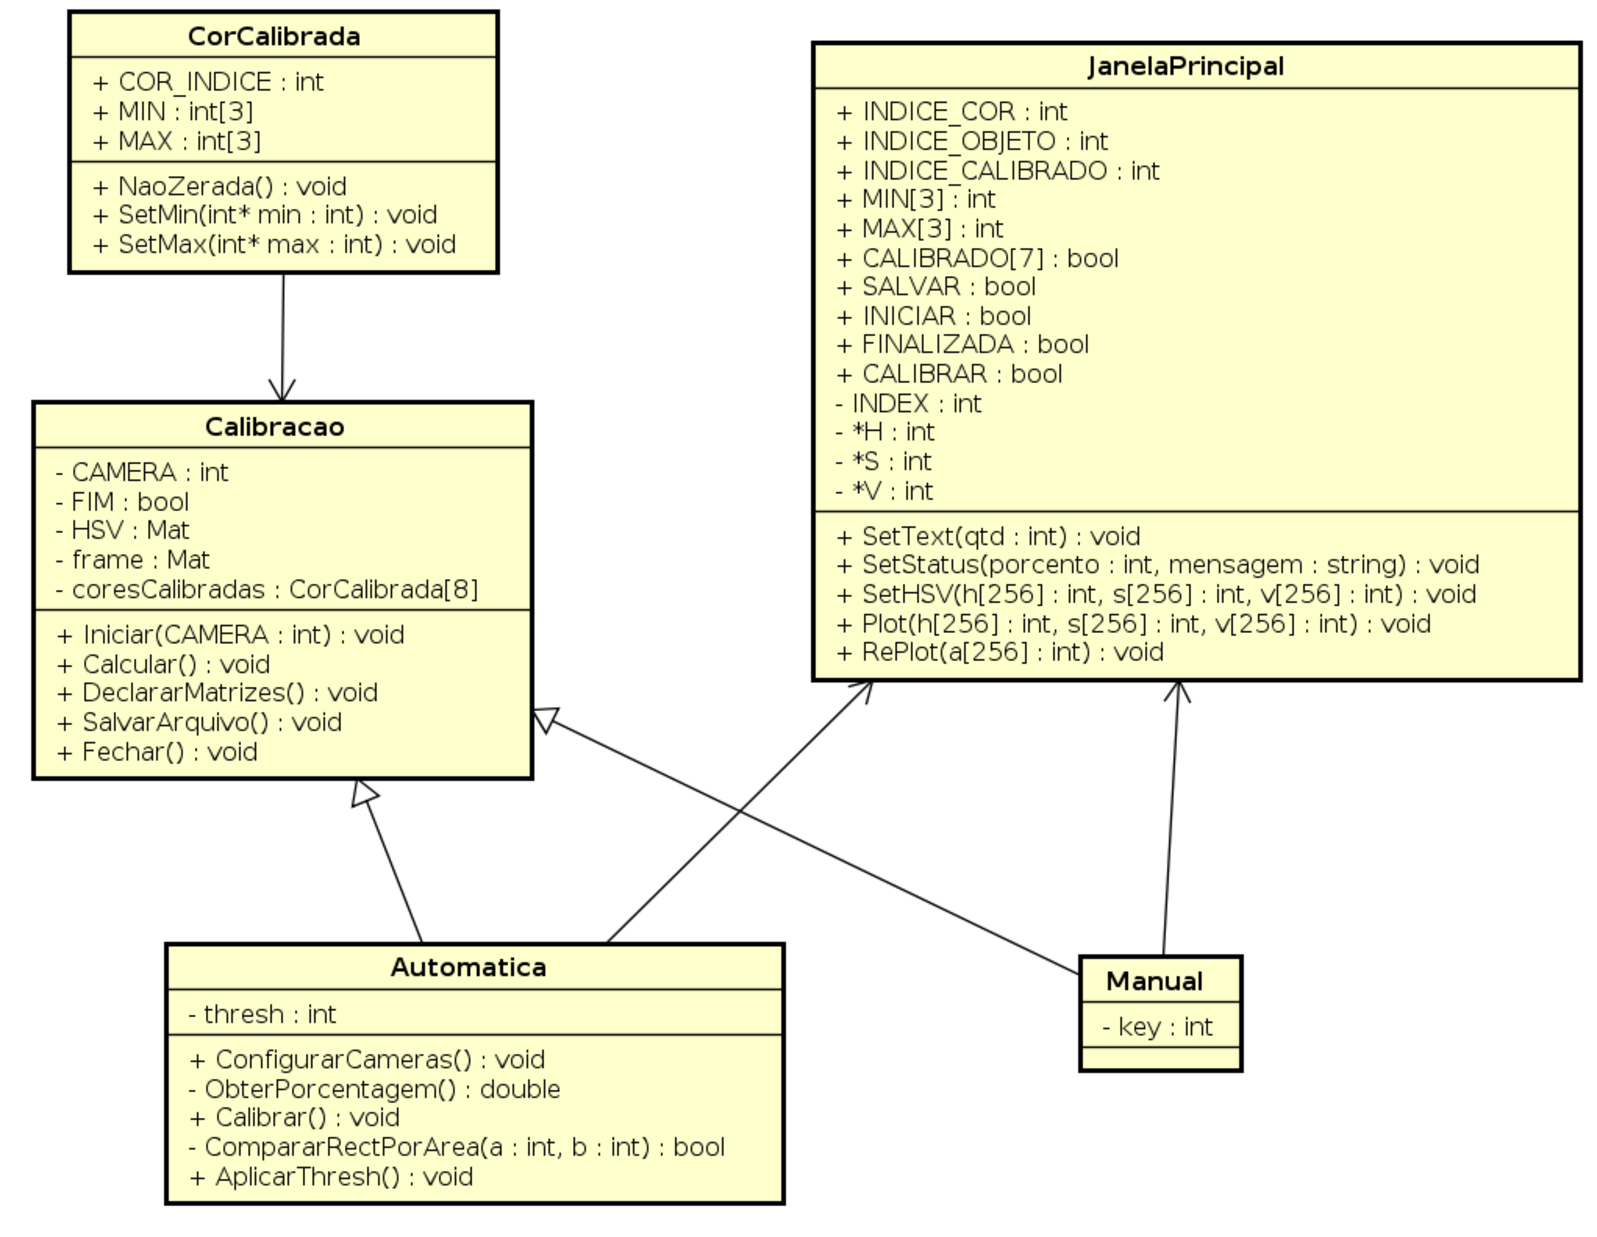
\includegraphics[width=0.5\textwidth]{diagramadeclasse.pdf}
	 	\caption{Diagrama de Classes do projeto}
	 	\label{Diagrama De Classe}
	 \end{figure}\newpage


	\subsubsection{Main}
	Classe principal onde ocorre aquisição de imagem, seleção de cores, contagem de ocorrência HSV, entre outros.
	
	
	\begin{description}
	\item [void SalvarArquivo()]
		Método sem retorno nem parâmetros, é neste método que o arquivo cores.arff é gravado com os valores da calibração.
	\item [void CalcularHSV(cv::Point ini, cv::Point fim)]
	Método sem retorno que recebe o ponto inicial e final da seleção da cor. Dentro desse método a imagem é convertida para o modelo de cores HSV e então são feitas as contagens de ocorrência dos valores HSV em cada pixel e adicionado ao seu vetor correspondente.
	\item [void mouseHandler(int event, int x, int y, int flags, void *param)]
	Método sem retorno com parâmetros de movimentação do mouse. Esse método segue o modelo especificado pela biblioteca OpenCV. Este método é onde são manipuladas as entradas do usuário via mouse. É onde são identificados a seleção do ponto inicial, feito então uma borda ao redor da seleção, e identificada o ponto final da seleção da cor. É nesse método que é chamado o método CalcularHSV.
	\item  [void DeclararMatrizes()]
	Método sem retorno e sem parâmetros. Neste método os vetores de H, S e V são limpos para então ser feita a calibração de uma outra cor.
	\item [void Calibracao(int argc, char **argv)]
	Método sem retorno que possui como parâmetros argc, que é um inteiro que que possui o total do número de argumentos que a classe foi executada na linha de comando, e argv que são os parâmetros usados na execução do programa na linha de comando, que serão usados para a execução da interface gráfica. Neste método são inicializados a câmera e a interface gráfica, e assim inicializando o processo de calibração e até que a mesma seja finalizada seja finalizada. 
	\item [void ThresholdImagem()]
	Método sem retorno e sem parâmetros onde é mostrado o resultado da calibração. Nele são levados em consideração os mínimos e máximos de cada cor e então feito um Threshold, um método onde são separados os grupos de cinza que formam os objetos da imagem e assim separar somente os objetos desejados.
	\item [int main(int argc, char **argv)]
	Método sem retorno que possui como parâmetros argc, que é um inteiro que que possui o total do número de argumentos que a classe foi executada na linha de comando, e argv que são os parâmetros usados na execução do programa na linha de comando. Neste método é invocado o método Calibração e após a finalização deste método é invocado o método ThresholdImagem(), para mostrar o resultado final.
	\end{description}
	\subsubsection{MainWindow}
	Interface gráfica onde são mostrados ao usuário as ocorrências de cada cor e obtidas as interações com o usuário por meio de seleção dos mínimos e máximos de cada um dos valores de HSV.  
	\begin{description}
		\item [void SetHSV(int h[256] , int s[256], int v[256])] Método chamado pela Main para passar os valores de ocorrência de HSV para a interface gráfica.
		\item[ void Plot(int h[256] , int s[256], int v[256])]
		 O método Plot é chamado pelo meto SetHSV e faz a inicialização dos gráficos de valores e sua exibição.
		\item [void RePlot(int a[256])]
		 Apos seleção via Slider ou Entrada de texto, o método RePlot atualiza a exibição do gráfico em questão.
		\item [void TabChangedTo(int index)]
		 Método que lida com a mudança das abas do gráfico.
		\item [void ComboChanged(int index)]
		 Método que lida com a mudança da cor para calibração no ComboBox.
		\item [void IniciarCalibracao()]
		Método que inicia a calibração.
		\item [void SalvarCalibracao()]
		Método que salva a calibração da cor atual.
		\item [void FinalizarCalibracao()]
		Método que finaliza a calibração.		
		\item [void setMaxTextInt(int value)]
		 Método que lida com alteração do valor Máximo na área de texto e atualiza tanto o gráfico quando o Slider.
		\item [void setMaxSliderValue()]
		 Método que lida com alteração do valor Máximo no Slider e atualiza tanto o gráfico quando a área de texto.
		\item [void setMinTextInt(int value)]
		 Método que lida com alteração do valor Minimo na área de texto e atualiza tanto o gráfico quando o Slider.
		\item [void setMinSliderValue()]
		  Método que lida com alteração do valor Minimo no Slider e atualiza tanto o gráfico quando a área de texto.

	\end{description}
	\subsubsection{CorCalibrada}
	Classe Objeto que guarda valores mínimos e máximos.
	\newpage

	\section{Fluxo do Sistema}
	O sistema pode ser basicamente divido em 4 etapas. Inicialização, Abertura do Programa, Calibração e Armazenamento. Para um melhor intendimento da execução do programa, seguem abaixo o diagrama de fluxo. 
		\begin{figure}[!h]
			\centering
			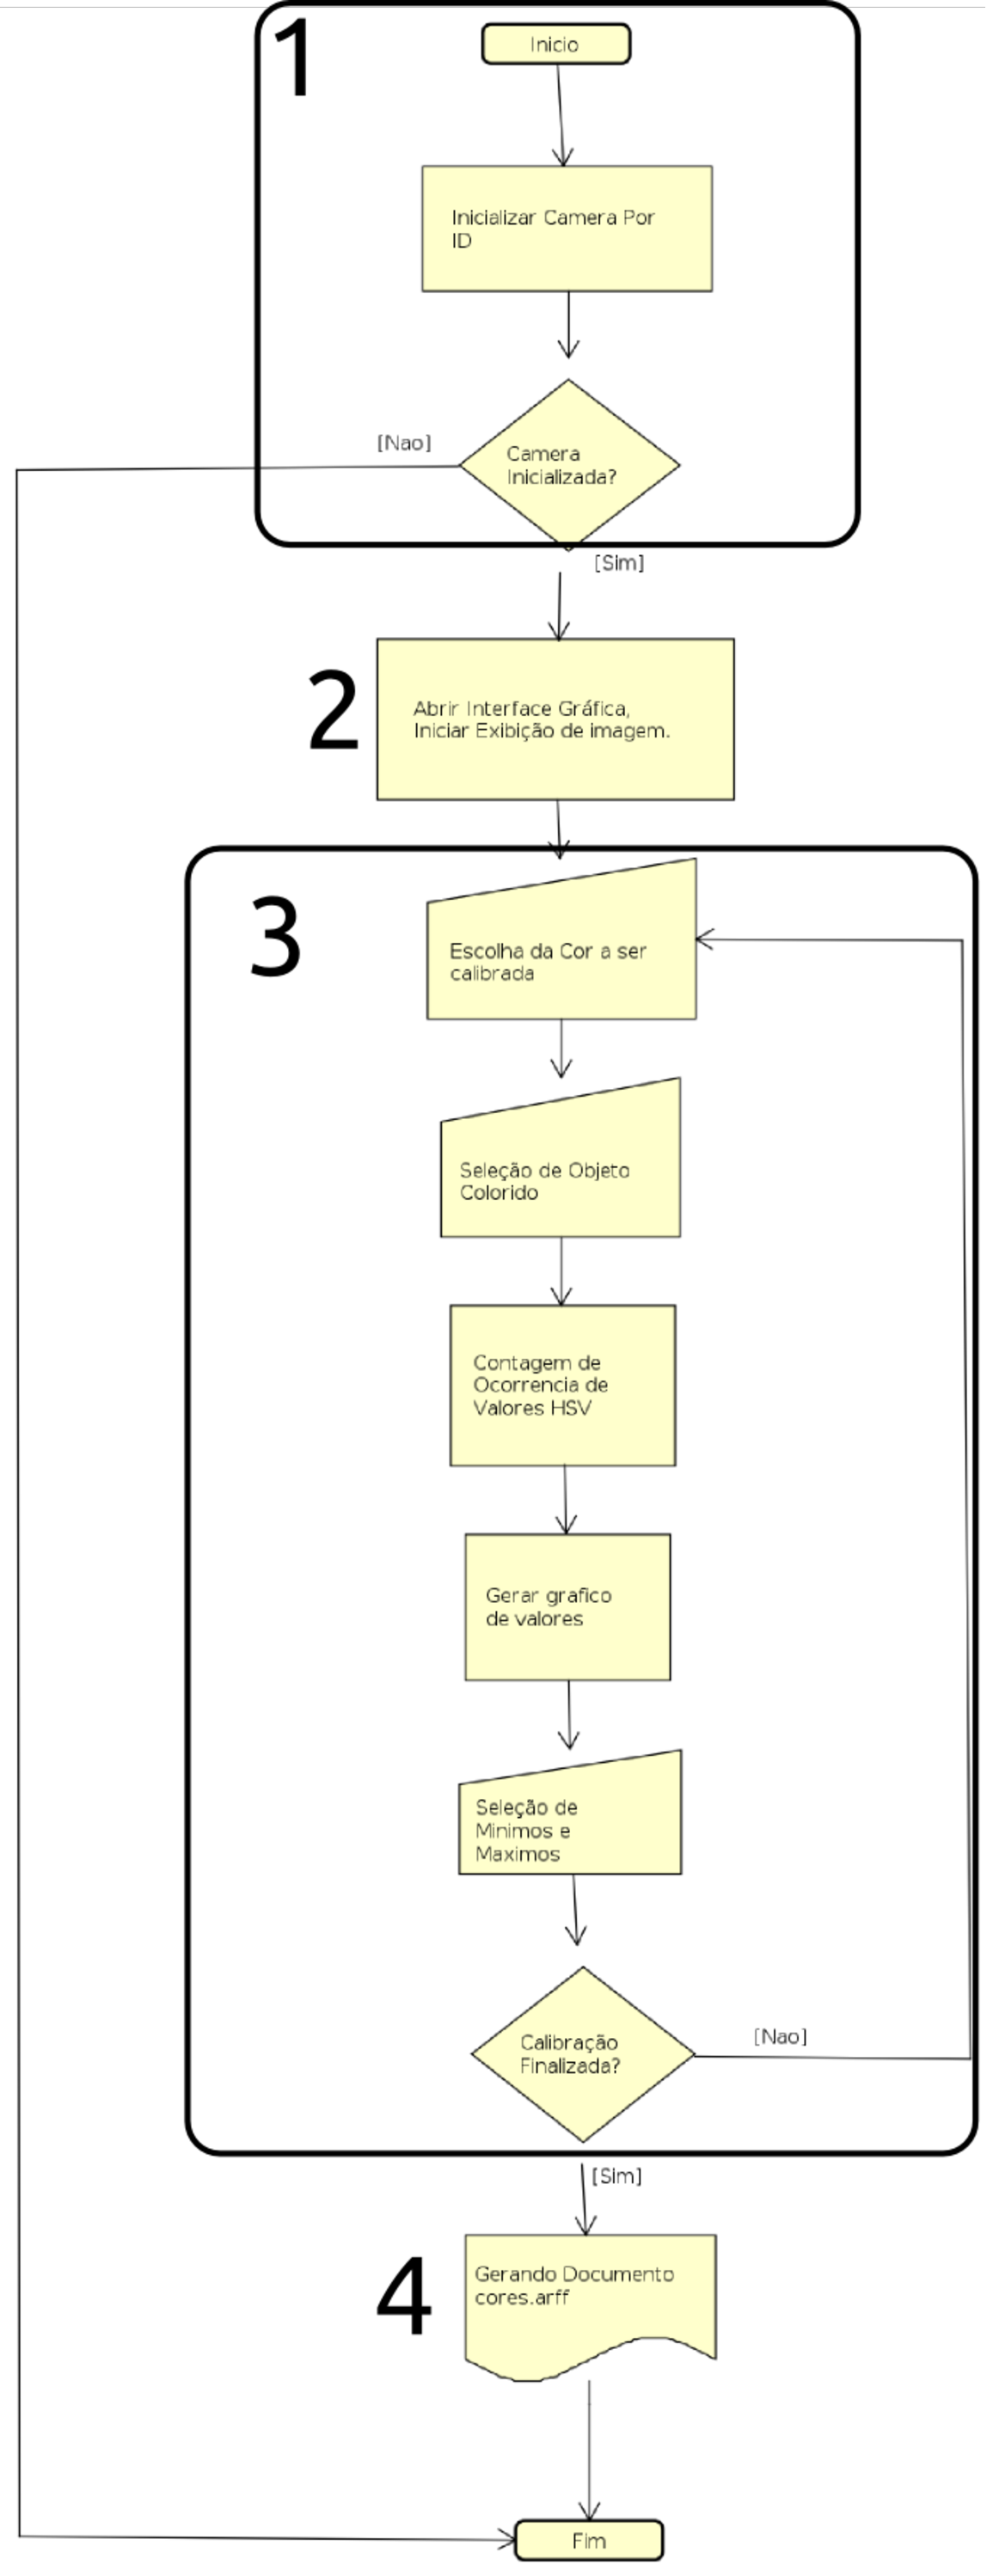
\includegraphics[width=0.45\textwidth]{DiagramaDeFluxo.pdf}
			\caption{Diagrama de Fluxo}
			\label{FlowCHart}
		\end{figure}
		
	\subsection{Etapa 1 - Inicialização}	
	Nesta etapa são declaradas todas as variáveis necessárias para execução do sistema, tanto da interface gráfica quanto da parte de processamento da imagem. Também é nesta etapa que se verifica a câmera esta disponível ou não. Caso a câmera não esteja disponível o sistema não é inicializado.
	
	
	\subsection{Etapa 2 - Abertura do Programa}		
		Após ter sido inicializado com sucesso o programa dispõe sua interface gráfica que é separada entre 2 janelas, a Janela 1, Gráfico, e a Janela 2, Seleção de Cores, detalhadas no Capítulo 4, sendo então possível iniciar o processo de calibração. 

\subsection{Etapa 3 - Calibração}		
			Esta etapa é onde ocorre a maior parte do sistema. O processo de calibração ocorre em um laço finito, até que esteja completa a calibração das cores desejadas e está subdividida em: Escolha da Cor, Seleção do Objeto Colorido, Contagem de Ocorrência HSV, Gerar Gráfico, Seleção de Mínimos e Máximos.
			
\subsubsection{Escolha da Cor}
			 Na Janela 1, utilizando o método de entrada disposto é escolhida a cor à ser calibrada. No momento estão disponíveis para calibração as cores: Amarelo, Azul, Ciano, Laranja, Verde, Vermelho, Rosa e Roxo, e seus índices de 0 a 7, correspondentemente. 
	\subsubsection{Seleção do Objeto Colorido}
	Apos a cor escolhida é então necessário que se selecione o ponto que obtenha a mesma na Janela 2. Essa seleção é feita usando pontos inicial e final que sera obtido quando o mouse é clicado na posição inicial e arrastado até a posição final. Apos selecionada a cor é então chamado o método que faz a contagem da ocorrência dos valores HSV em cada pixel.

	\newpage
	\subsubsection{Ocorrência HSV}
	O primeiro passo da calibração é a varredura do(s) ponto(s) selecionado(s) pelo usuário, encontrando os valores HSV de cada pixel, e esses adicionados ao vetor de ocorrência. 
	Quando o método é chamado são passados por referencia os pontos inicial e final da varredura, o frame da imagem é convertido para HSV e então feito sua ocorrência. 

		\begin{lstlisting}
		// Método de varredura de pixel e ocorrencia de HSV
		cv::cvtColor(frame, hsv, CV_RGB2HSV);
		for (int y = ini.y; y < fim.y; ++y) {
			for (int x = ini.x; x < fim.x; x++) {
			pixel = hsv.at<cv::Vec3b>(y, x); 
			H[pixel.val[0]]++;
			S[pixel.val[1]]++;
			V[pixel.val[2]]++;
				} 
		}	\end{lstlisting}
	\subsubsection{Gerar Gráfico}
	Após a seleção da cor, o usuário escolhe calibrar a cor, a geração dos valores só é feita quando o usuário apertar o botão "Calibrar", pois pode ser que a cor a ser calibrada esteja em mais de um ponto da imagem.
	Quando os pontos com cor são selecionados um gráfico dos valores de H, S e V são gerados e mostrados para usuário. 
	\subsubsection{Seleção de Mínimos e Máximos}
	Mínimos e Máximos são selecionados com interação do usuário. Após salvos são armazenados em variais dentro do programa. Quando toda a calibração é terminada o programa finaliza o laço de repetição do processo.
\subsection{Etapa 4 - Armazenamento}
Nesta etapa é onde é gerado e armazenado em disco o arquivo cores.arff onde os valores cada cor estão separados em duas linhas, a primeira linha contem os valores mínimos e a segunda os máximos.
	\newpage
	
	
